\documentclass[11pt]{article}

% basic packages
\usepackage[margin=1in]{geometry}
\usepackage[pdftex]{graphicx}
\usepackage{amsmath,amssymb,amsthm}
\usepackage{william}
\usepackage{tikz}
\usetikzlibrary{arrows.meta, positioning}

% page formatting
\usepackage{fancyhdr}
\pagestyle{fancy}

\renewcommand{\sectionmark}[1]{\markright{\sffamily #1}}
\renewcommand{\subsectionmark}[1]{}
\lhead{\bfseries\thepage \ \ \nouppercase{\rightmark}}
\chead{}
\rhead{}
\lfoot{}
\cfoot{}
\rfoot{}
\setlength{\headheight}{14pt}

\linespread{1.03} % give a little extra room
\setlength{\parindent}{0.2in} % reduce paragraph indent a bit
\setcounter{secnumdepth}{2} % no numbered subsubsections
\setcounter{tocdepth}{2} % no subsubsections in ToC

\begin{document}

% make title page
\thispagestyle{empty}
\bigskip \
\vspace{0.1cm}

\begin{center}
{\fontsize{22}{22} \selectfont Lecture Notes on}
\vskip 16pt
{\fontsize{36}{36} \selectfont \bf \sffamily Machine Learning}
\vskip 24pt
{\fontsize{18}{18} \selectfont \rmfamily Will Lancer} 
\vskip 6pt
{\fontsize{14}{14} \selectfont \ttfamily will.m.lancer@gmail.com} 
\vskip 24pt
\end{center}

{\parindent0pt \baselineskip=15.5pt}
\noin
Notes on machine learning. Each section is another ML course or paper
that I did. Links to the resources are included section by section.
Then there is my organization of the content as a whole (coming after
I familiarize myself with the landscape of AI/ML).

% make table of contents
\newpage
\microtoc
\newpage

% main content
\section{Kaggle's intro course and Google's \emph{Introduction to Machine Learning}}

See the \href{https://github.com/will-lancer/notes/Computer_Science/Python/Python.pdf}{notes} 
on Python to refresh on the necessary NumPy and Pandas
to follow the example below.

\begin{iidea}
    [Basic terminology]
    Your data points are called
    \vocab{examples}, your parameters are called \vocab{features},
    and your desired prediction parameter is called the \vocab{label}.
    There are a few distinctions in machine learning:
    \begin{itemize}
        \item \vocab{Supervised learning} vs. \vocab{unsupervised learning}. Supervised
        just means you give the model the right answer in the end,
        and unsupervised means you don't (doing that may not even be well-defined).
        \item Supervised learning: \vocab{regression} vs. \vocab{categorization}.
        Regression predicts a numerical value and categorization predicts
        a likelihood that the label is in a given category. You can have binary
        or multi-category categorification.
        \item \vocab{Reinforcement learning} (broader than supervised/unsupervised).
        Gives the model rewards/punishments based on actions peformed within
        its training environment.
    \end{itemize}
    The basic ML workflow is
    \begin{center}
    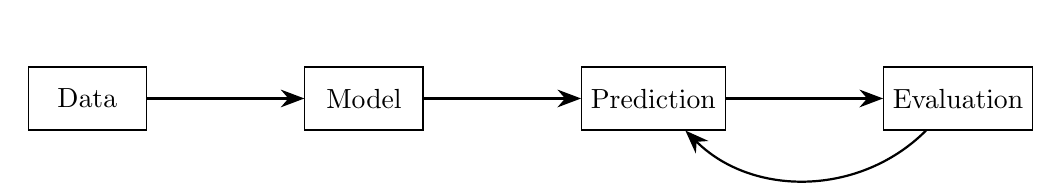
\begin{tikzpicture}[
        node distance=2cm,
        box/.style={rectangle, draw, minimum width=1.5cm, minimum height=0.8cm, align=center},
        arrow/.style={-{Stealth[length=3mm]}, thick}
    ]
        % Main flow nodes
        \node[box] (data) {Data};
        \node[box, right=of data] (model) {Model};
        \node[box, right=of model] (prediction) {Prediction};
        \node[box, right=of prediction] (evaluation) {Evaluation};
        
        % Main flow arrows
        \draw[arrow] (data) -- (model);
        \draw[arrow] (model) -- (prediction);
        \draw[arrow] (prediction) -- (evaluation);
        
        % Feedback loop arrow
        \draw[arrow] (evaluation) to[bend left=45] (prediction);
    \end{tikzpicture}
    \end{center}
    where your prediction and evaluation cycles continue ad infinitum.
\end{iidea}


\begin{eexample}
    [The decision tree]
    This extended example is Kaggle's intro course. It will help us get familiar
    with the general process before going into deeper theory.
    We first need to make our data into a DataTable to do analysis on it.
    We can import it from a csv by using \verb|df = pd.read_csv(dataFilePath)|.
    We look through our data using \verb|df.describe()| and \verb|df.head()|.
    We now need to specify features and a label. We do this by
    \begin{verbatim}
        features = ['column1', 'column2', ..., 'columnN']
        # 'X' is the standard name for the vector of feature data
        X = df[features]
        # 'y' is the standard name for the label vector
        y = df['labelColumn']
    \end{verbatim}
    Then we use some machine learning magic to train this data on this data set.
    For the decision tree, we import the decision tree trainer and then run it on the
    data,
    \begin{verbatim}
        from sklearn.tree import DecisionTreeRegressor
    \end{verbatim}
    We then declare a decision tree regression model and train it
    on our data,
    \begin{verbatim}
        decisionTree = DecisionTreeRegressor(random_state = 1)
        decisionTree.fit(X, y)
    \end{verbatim}
    Now we can use this to predict things, so we can say things
    like \verb|decisionTree.predict()| or \verb|decisionTree.predict(X.head())|
    to get predictions. You can optimize the number of leaves in your
    decision tree by minimizing the \vocab{mean absolute error},
    which is defined as
    \begin{align*}
        {\rm MAE} = \frac{1}{N} \sum_i^N |\mathbf{y}_{\rm train} - \mathbf{y}_{\rm val}|.
    \end{align*}
    You can import the mean absolute error module from \verb|sklearn.metrics|
    like before,\\ \verb|import mean_absolute_error|.
    You can also import a train-test-split tool from\\
    \verb|sklearn.model_selection|
    to get some validation data from your training set.
\end{eexample}

That's it! That's our first basic ML model. Let's summarize what we did
in more abstract terms now:
\begin{itemize}
    \item We had a given cleaned data set to work with.
    \item We set up our data for processing by turning it into a DataTable.
    \item We used a given algorithm to train our model on this data.
    \item We tested our model on some validation data.
    \item We further refined this model by giving it an optimization condition---in this
    case, we were minimizing the $L^1$ norm (MAE) as compared to the validation data.
\end{itemize}

\noin
From this I will remind ourselves of a meta-level heuristic from King Ilya:
\begin{quote}
    \emph{The model just wants to learn}. All we did was set up data-processing,
    say which algorithm we were using, and get out of the model's way. Then it tried
    its best to learn given the training data we gave it. After checking its progress, we 
    then gave it another learning tool (the MAE); this gives the model a more precise way
    of telling whether things are right or wrong (i.e. there is some measure of magnitude
    which isn't present in a binary classifier). The model did everything difficult here: we
    just helped it along its way.
\end{quote}

A useful way of thinking about the difference between parameter correction and 
model correction.
\begin{eexample}
    [Inner-loop vs. outer-loop learning, and a physical analogy]
    The \emph{inner loop} is the model learning by itself, and the \emph{outer loop}
    is outside sources telling the model other ways to learn. This is the distinction between
    the model training itself on some set of training data vs. the validation and correction phase
    of learning. The model is doing inner loop learning, then you come in and do outer loop
    learning. Of course, human intervention is not necessary---one could imagine another AI
    telling the model to change something. But something has to come in and help this model
    do outer loop learning. There is some sense of discontinuity with model correction vs.
    parameter correction. 
    
    An analogy is electrostatic equilibrium: if you place two charged conductors
    in the vicinity of one another, they will continuously relax into equilibrium by minimizing
    $\mathcal{E} = 1/8\pi \int d^3 \bfr' \, \elec \cdot \mathbf{D}$. This is parameter correction. Model correction 
    would be you changing the material of the conductor. There is no continuous sense in which this occurs:
    you just change it and let things re-run.

    Another analogy is a kid learning how to ride a bike. The kid continuously adjusts their strategy
    in response to the optimization condition of balancing (i.e. keeping the COM over the supports):
    this is parameter adjustment. Then let's say the kid's dad comes in and gives him a smaller bike (he
    determined that the one he was riding was too big) and tells him to not try and pedal so fast (the kid was
    always trying to go to fast and thus was losing his balance too quickly), and tells him to go out there and
    try again. This is model correction.
\end{eexample}

\section{CS 231n}

This section of the notes follows Karpathy's \href{http://cs231n.stanford.edu}{CS 231n course}.
This is my first bonafide ML course.

\end{document}